\documentclass[a4paper,twoside]{article}

\usepackage{epsfig}
\usepackage{subfigure}
\usepackage{calc}
\usepackage{amssymb}
\usepackage{amstext}
\usepackage{amsmath}
\usepackage{tikz}
\usepackage{amsthm}
\usepackage{multicol}
\usepackage{pslatex}
\usepackage{apalike}
\usepackage{SCITEPRESS}
\usepackage[small]{caption}
\usepackage{color}
\usepackage{xfrac}

\subfigtopskip=0pt
\subfigcapskip=0pt
\subfigbottomskip=0pt

\begin{document}

\title{Improving physiological signal classification using logarithmic quantization & progressive calibration}

%Quantization and Calibration
%Logarithmic Quantization and Opportunistic Calibration for Physiological Signal Classifiers
%Quantization and Calibration for Efficient Physiological Signal Classifiers
%Towards Rapid Calibration of Physiological Signal Classifiers

%\title{Strategies for the quick calibration of sensor-driven systems with low computational overhead}

\author{\authorname{Anonymized Authors}
\affiliation{Anonymized Institution}
\affiliation{Anonymized Institution}
\email{Anonymized Emails}
}

%\author{\authorname{Nick Merrill\sup{1}, Thomas Maillart\sup{1}, Benjamin Johnson\sup{2} and John Chuang\sup{1}}
%\affiliation{\sup{1}School of Information, UC Berkeley, Berkeley, California, USA}
%\affiliation{\sup{2}Carnegie Mellon University}
%\email{ffff@berkeley.edu,,,john.chuang@berkeley.edu}
%}

\keywords{bio-signal processing, signal quantization, logarithmic binning, user calibration, brain-computer interface}
%\keywords{BCI, Mobile, Ubiquitous Computing}

% make this cooler and more accessible
\abstract{Physiological computing applications rely on time series sensor data, the meanings of which vary widely between users and change over time. Application designers face a tradeoff between computational complexity, calibration time, and classification accuracy. We describe a quantization technique for electroencephalograph (EEG) signals which increases the computational speed associated with training a machine-learning based classifier without a significant detriment to the system's accuracy. We test this technique on a brain-computer interface (BCI) that uses a single EEG sensor, and find that a progressive calibration strategy achieves high accuracy in 86.6\% of subjects with under five minutes of training, and in 100\% of subjects with under 15 minutes. We discuss implications for consumer-ready BCI and for physiological computing applications generally.}

\onecolumn \maketitle \normalsize \vfill

\section{\uppercase{Introduction}}
\label{sec:introduction}

\noindent Physiological data do not carry universal meanings. While the movement of a computer mouse can be mapped to the position of a cursor in a straightforward manner, the expression of bio-signals varies widely between individuals, and often changes within individuals over time. Brain-computer interface (BCI) serves as a good example of this phenomenon: regular calibration and re-calibration are essential due to the personal and non-stationary nature of neural signals \cite{dornhege_toward_2007,mcfarland_brain-computer_2011}.

Supervised learning algorithms have enabled systems to adapt to users' personal physiology after a calibration period. In BCI, this approach has yielded proof-of-concept systems ranging from brain-controlled keyboards and wheelchairs to prosthetic arms and hands \cite{blankertz_note_2007,millan_combining_2010,d._mattia_brain_2011,hill_practical_2014,campbell_neurophone:_2010}. 

% For similar devices to find use outside of the lab, they  minimize both the size of our sensing devices and the amount of time users spend calibrating the interface. % minimal number of sensors + limited computational power on mobile devices % while still accurate and quick-to-calibrate

% BCIs often require upward of an hour to calibrate to their users, with close supervision by researchers, and may require regular recalibration due to the nonstationary nature of EEG signals. \cite{vidaurre_fully_2006,vidaurre_co-adaptive_2011,blankertz_non-invasive_2007} Recent work has come close to eliminating traditional calibration, though these techniques have not yet been applied to consumer headsets. \cite{kindermans_true_2014}

Moving from laboratory settings into the real world, these systems will have fewer and less sensitive sensors due to cost, ergonomic and aesthetic considerations. They will also process noisier signals as data acquisition will occur while people are engaged in everyday activities, walking, talking, sleeping, and so on. As an additional challenge, computational complexity, measured by both storage and processing requirements, may be limited by the mobile and wearable computing architectures on which these systems will be deployed. 

% This leads us to pose the following research question: how fast and with how little computational power can we build a practical BCI?

In this paper, we study how the processing of physiological signals and the strategy for user calibration can impact the performance of a machine-learning based bio-signal classification system. We use signals acquired from a low-cost, mobile electroencephalograph (EEG) device with a single sensor. Prior to classification, how can we operationalize the tradeoff between computational complexity and classification accuracy at the signal processing step? Given a well-tuned classifier, is it possible to realize user calibration on the order of minutes rather than hours or days?

%How can we process EEG signals such that we minimize the computational expense of classification while maximizing the system's accuracy? Is a computationally efficient signal processing technique compatible with a user-calibration protocol that achieves ``BCI literacy'' across all subjects on the order of minutes rather than hours or days?

We propose a novel signal quantization technique that applies logarithmic binning to power spectrum data from a single EEG electrode. We find that this technique can increase the computational speed of a classification-based BCI by 450\% compared to uncompressed data without significant detriment to accuracy. In conjunction with a progressive user-calibration protocol, in which candidate mental gestures are tested ``on demand'' in order to minimize calibration time, we calibrate 86.6\% of users to a threshold of BCI control in under five minutes of training data, and 100\% of users in under 20 minutes. 

This paper is organized as follows. We discuss related works in Section \ref{sec:related}, and provide a summary of the dataset in Section \ref{sec:data}. We describe our signal quantization method in Section \ref{sec:quantization}, and quantify its effect on classifier speed and accuracy in Section \ref{sec:quantization_eval}. We evaluate a user calibration strategy in Section \ref{sec:calibration_eval} before concluding.

\section{\uppercase{Related Work}}
\subsection{Brain-computer interface ``in the wild''}

\noindent Wider adoption of BCI systems relies on two main streams of research: (i) the development of ergonomic sensors suitable for use in naturalitic settings and (ii) the ability to adapt lab-developed BCI strategies to the new constraints that these sensors impose on our data processing abilities. 

% TODO: cite surveys of devices-- there's a survey of EEG hardware from wheelchairs from south africa but maybe tehre's something moe recent
% TODO: study comparing consumer grade to medical grade EEG ---- just read one recently, it's in my zotero
Many inexpensive, comfortable EEG devices have come to market, most of which use ``dry'' electrodes that do not require special gels. Compared to their lab-based counerparts, these devices have many fewer electrodes, thus limited spatial resolution, and produce significantly noisier signals \textcolor{red}{\bf (is there a benchmark available in the literature?)}. Regardless, past work has demonstrated several mobile-ready BCI systems that use these scanning devices, and the Neurosky MindSet in particular (the headset used in this study - a single, dry EEG electrode placed roughly at FP2, which connects wirelessly to phones and computers, and sells for roughly 100USD) has been used to succesfully detect emotional states, event-related potentials (ERP), and to employ brain-based biometric authentication \cite{crowley_evaluating_2010,grierson_better_2011,adams_i_2013}.  However, the use of consumer EEGs for the direct, real-time control of software interfaces has proven more difficult \cite{carrino_self-paced_2012,larsen_classification_2011}. We expect significant improvements from consumer-grade EEG devices in the near future, with more sensors and better signal quality (e.g. Interaxon Muse, Melon headband, Emotiv Insight); however, we expect the signal from these devices will remain noisier than lab-basde counterparts, as people will be wearing and using them while moving, and in uncontrolled environments with ambient electromagnetic signals interfering with endogenous biosignals. \textcolor{red}{\bf Mobile systems require reducing the bandwidth (currently 1 megaoctet per dry EEG sensor sampling at 512 Hz) <-- why/what does this mean? }.

To transition BCI from the lab into naturalistic environments, we must squeeze more signal out of fewer, and less reliable, sensors. Furthermore, since BCIs are envisioned largely as always-available input devices, they will likely be deployed on mobile processors and perhaps even embedded processing systems; our computational resources may be more similar to that of a smartphone than of a desktop workstation, and it is feasible that we may need to do some processing ``in the cloud'' (ie., on a more powerful server to which the client sends data over the network, similar to the way Apple's Siri processes voice data). For effective BCI to occur in these environments, we must extract signal in a maximally efficient way so as to limit our computational footprint, and perhaps even to minimize the size of data if we wish to ship it to an external server.

\subsection{Statistical signal processing in EEG-based BCI}

\noindent BCI systems generally aim to recognize a user's mental gestures as one of a finite set of discrete symbols, a problem that can be thought of as a pattern recognition task \cite{lotte_review_2007}. The difficulty of this task stems primarily from the variable and non-stationary nature of neural signals: the ``symbols" we wish to identify are expressed differently between individuals, and even vary within individuals from trial to trial \cite{vidaurre_fully_2006,vidaurre_machine-learning-based_2011}. 

In order to compensate for variability in BCI signals, recent work has leveraged adaptive classification algorithms to distinguish between mental gestures \cite{lotte_review_2007,vidaurre_machine-learning-based_2011} \textit{steal some lines introing classificatino algos............maybe steal a line explaining what a classifier is in the context of a BCI system, and how we train one......}.  In classification algorithms generally, larger feature vectors require that an exponential increase in the amount of data needed to describe classes, a property known as ``the curse of dimensionality'' \cite{jain_statistical_2000,raudys_small_1991}. Traditionally, BCI applications rely on dense, high-diemsnional feature vectors produced by multi-electrode scanning caps with high temporal resolution, so dimensionality represents a major bottleneck in training classification algorithms. This bottleneck threatens the responsiveness of BCI from a user experience standpoint and places high requirements on end users' hardware.

\subsection{Online, co-adaptive calibration}

\noindent Learning to control a BCI system involves more than an adaptive software algorithm. Shenoy et al (2006) frame BCI learning as a cooperation between two adaptive systems: the BCI's algorithms and the human user \cite{shenoy_towards_2006}.  By building interfaces in which the user and the BCI ``co-adapt'' during an interactive calibration step, past work has turned BCI novices into competent users over the course of hours instead of days or weeks, and without manual calibration by a researcher \cite{vidaurre_fully_2006,vidaurre_co-adaptive_2011,vidaurre_machine-learning-based_2011}. 
Past work on co-adaptive BCI has used a several-step approach in which the system feeds preprocessed data to an adaptive classifier, which uses new and past data to optimize and recalculate itself, either during intermittent, offline steps or continuously online \cite{vidaurre_fully_2006,shijian_lu_unsupervised_2009,das_unsupervised_2013}. During calibration, users perform ``labeled'' (that is, known) mental gestures in order to produce samples for the classifier. Meanwhile, the classifier performs various experiments in which it attempts to establish which features of the data are most informative. Systems may generate multiple models in parallel and combine their decisions democratically (an ``ensemble approach''). After several calibration steps, the system is able to estimate the user's control by assessing its model's accuracy on samples it has already recorded.

\subsection{Co-adaptive BCI in naturalistic settings}

% thomas's note on "change for the same subject over time": Since you have mentioned this issue in the manuscript, you might want to test robustness of our classifier over two different sessions. If remember well, we have data for this.
\noindent For the control of interface systems, it is crucial that mental gestures be actuated intentionally, and that the system's interpretation be immediately verifiable by the user. \cite{mcfarland_brain-computer_2011} \textit{Maybe a line here about how the system needs to be fast for responsiveness} Efficient calibration is particularly crucial for real-world use, as EEG signals vary between subjects, and could even change within the same subject over time. From a technical standpoint, calibration amounts to the training and re-training of one or several adaptive algorithms. Calibration can be processing-intensive on a mobile device, especially if the system is computing multiple candidate models. This requires a great deal of online signal processing, which entails not only the computational time required to train the classifier but also the space required to handle the data and the time required to read and write the data from memory or from disk.

% drop another hint about embedded sensors and doing stuff in the cloud


\section{\uppercase{Dataset}}

The data used in this experiment were taken from a previous study. The anonymized dataset consists of power spectrum time series data recorded by the software from the Neurosky MindSet headset from 15 subjects, who were students at UC Berkeley, performing mental tasks. Participants performed each of the seven mental tasks, enumerated below, ten times. Each of the ten trials lasted ten seconds.

The seven mental tasks were: focusing on breathing; imagining moving one's right index finger; imagining moving one's body to repeatedly perform a sports-related movement of the subject's choice; imagining singing a song or reciting a passage; listening to a tone with eyes closed; choosing a color (red; green; yellow or blue) and counting how many times one's chosen color appears on a screen; choosing any thought to use as a ``password''.

%\section{\uppercase{Method}}

This section details the signal extraction technique that this study evaluates and describes the machine learning classifier used in our binary BCI.

\subsection{Signal extraction}

\subsubsection{Compressing power spectra in the temporal dimension}

For each bin of 1/4 Hz, we compute a median value out of the n power spectra generated for one sample. We obtain a discrete probability density function (PDF) with each bin being the median of the corresponding bins in the n power spectra. At this stage, we have a discrete PDF of 1024 bins for the whole sample. This method represents a ``stacking" of several PDFs into one PDF that represents the statistical average of all the others.

\subsubsection{Logarithmic binning}

Binning the PDF is a simple way to ``quantize'' the information contained in the original power spectrum. By taking the median of several bins, we are left with a single bin that compresses the information of its neighbors. For instance, four contiguous bins (1-1.25,1.25-1.5,1.5-1.75,1.75-2) have the values (4,4,5,5) the value resulting from combining these values into one bin would be 4.5. 

It is desirable to arrange the bins such that they provide relevant information on the whole distribution. Because the PDF is heavy-tailed, one way to do this efficiently is to arrange the compression bins in a logarithmic fashion. 

% thomas notes: I think here is the originality of the method: we take all the power spectrum with one advantage and one disadvantage. The advantage is that we have a much larger spectrum to characterize and classify tasks, at the cost of probably more pollution from non-EEG signal from the environment, from muscles, etc.]}

\begin{figure}[!h]
  \vspace{-0.2cm}
  {\epsfig{file = Figures/binned_EEGPowerSpectrum.png, width = 6cm}}
\caption{In double logarithmic scale, the original 1024 bins (blue dots) of the PDF obtained from averaging the n power spectra of one recording, and the resulting ``quanitized''  PDF with a resolution of 100 log-bins. The quantized PDF preserves very well the structure of the original, 1024-point PDF. }
\label{binnedEEGpowerspec}
\vspace{-0.1cm}
\end{figure}

In summary, we build a probability density function of brain frequencies as captured by the Neurosky hardware, from the n power spectra of each sample. We then used a log-binning method to reduce the 1024 bins from the original power spectrum to an arbitrary smaller number of log-bins (e.g., 100 log-bins on the Figure). This method makes a sort of statistical averaging by stacking, and then compresses the result in way that it is easy to use in a classifier.


% {\bf NB:} I believe that the classifier does well because it can efficiently capture the overall level of activity for all log-bins, but also more local deviations. On the figure, we can see some local peaks mostly between $10^1$ and $10^1.5$, but in all other parts of the PDF though in a less visible way. I believe these deviations are quite unique and can make the difference in the classifier. We should indeed check this further if we want to understand to origins of the good results.

% {\bf Side note:} one way to investigate further would be to see indeed to what extent the ``compression", i.e. the small number of log-bins, affects the quality of the classifier. Another quite promising further research direction, would be to determine the minimum number of n power spectra, which should be taken into account to reach a target level of correct classification. This would be useful to determine what should be the most adequate sample size for a certain level of identification. This level might of course vary as a function of subjects and tasks.

%-----------


% \textcolor{red}{\bf [Maybe a schema would be great to help the reader get the point quickly]}


\subsection{Classifying EEG signals}


In this study, we build a binary BCI using a support vector machine (SVM) classifier, which we train individually for each subject. SVMs work by drawing a discriminatory boundary (a ``hyperplane'') between training examples such that the margin of the hyperplane is maximized for all examples in the set. (For more on the use of SVMs in BCI: \cite{garrett_comparison_2003,grierson_better_2011}). 

\subsubsection{LibLinear}
We use LinearSVC, \cite{fan_liblinear:_2008} a wrapper for LibLinear exposed in Python through the ScikitLearn library. \cite{pedregosa_scikit-learn:_2011} We chose LinearSVC because BCI classification problems are generally presumed to be linear  \cite{garrett_comparison_2003,lotte_review_2007}, and because LibLinear's underlying C implementation boasts among the fastest train- and test-time performance among state-of-the-art solutions. \cite{fan_liblinear:_2008} For the SVM's paramaters, we use a squared hinge loss function, which maximizes the margin for greater generalizability, and a hyperparameter of 100, found through a ``grid search'', or an exhaustive search through a randomly selected sample of our dataset. 

\subsubsection{Cross-validation}

\textcolor{red}{\bf explanation of why we bother with cross validation, and what it means to estimate the accuracy of a classifier }

We use ScikitLearn's built-in cross-validation toolkit, which performs each of the seven cross-validation steps using different splits of trial data in the training and testing sets. 


\section{\uppercase{Signal Quantization For Rapid Classification}}
\label{sec:quantization}

%We are interested in minimizing computational expense of classifying mental gestures. This study investigates a signal quantization technique that reduces the size of EEG data for fast classification but retains high accuracy.

\noindent Our objective is to maximize the accuracy of the classifier while minimizing its computational expense. One way to reduce the computational requirements of a classifier is to reduce the size of the feature vectors on which it is trained and tested. We propose a signal quantization method that allows us to directly adjust the size of feature vectors. Since vector size directly impacts the runtime of the classifier, this technique operationalizes the tradeoff between computational speed and accuracy.

%Generally, we seek to maximize our system's classification accuracy while minimizing its computational expense. One way to reduce the computational requirements of a SVM classifier is to reduce the size of the feature vectors on which it is trained and tested. Our signal quantization method allows us to directly adjust the size of feature vectors by changing the signal's resolution (see 3.1), though lowering the resolution of feature vectors could negatively effect the classifier's performance.

%\subsection{Compressing power spectra in the temporal dimension}

We average the power spectrum time series in the temporal dimension and compute a discrete probability density function (pdf) from the resulting power spectrum in which each component is the mean of its corresponding frequency components through time. This results in a discrete pdf with 1024 components
for each trial, which can be quantized as described in the following section.

%First, we compute an average of all the power spectra associated with a recording. We obtain a discrete probability density function (PDF) in which each bin is the mean of its corresponding bins through time. At this stage, we have a discrete PDF of 1024 bins for the entire n second recording. 

\subsection{Logarithmic Binning}

Since EEG activity is associated with frequencies from 1-40Hz, it is generally presumed that this range contains the majority of relevant signal. However, this frequency range can be polluted with non-neural signals \cite{ball2009signal}, and we do not rule out the possibility that useful signal exists outside this frequency range as well. Muscular activity, for example, might be correlated with mental gestures in some cases. In order to exploit the entire frequency spectrum while preserving our bias toward known sources of useful signal, we select log-spaced data bins through the logarithm of the frequency range. Figure \ref{binnedEEGpowerspec} shows an example of logarithmic binning with 65 bins. The original, 1024-point pdf is compressed more than 10 times, but its original structure is well-preserved.

Data binning offers a simple way to quantize the information contained in the full signal. By taking the mean of several adjacent points in the pdf, we are left with a single bin that represents the local area of spectrum. For example, four contiguous frequencies (1Hz, 1.25Hz, 1.5Hz, 1.75Hz) of the values (4, 4, 5, 5) average into a single bin with the value 4.5. The number of bins can be adjusted to produce feature vectors of different sizes. This vector, which highlights the statistical properties of the power spectrum for each mental task, can be used as an input of variable size to the classifier.

\begin{figure}[!h]
  \vspace{-0.2cm}
  \centering
  {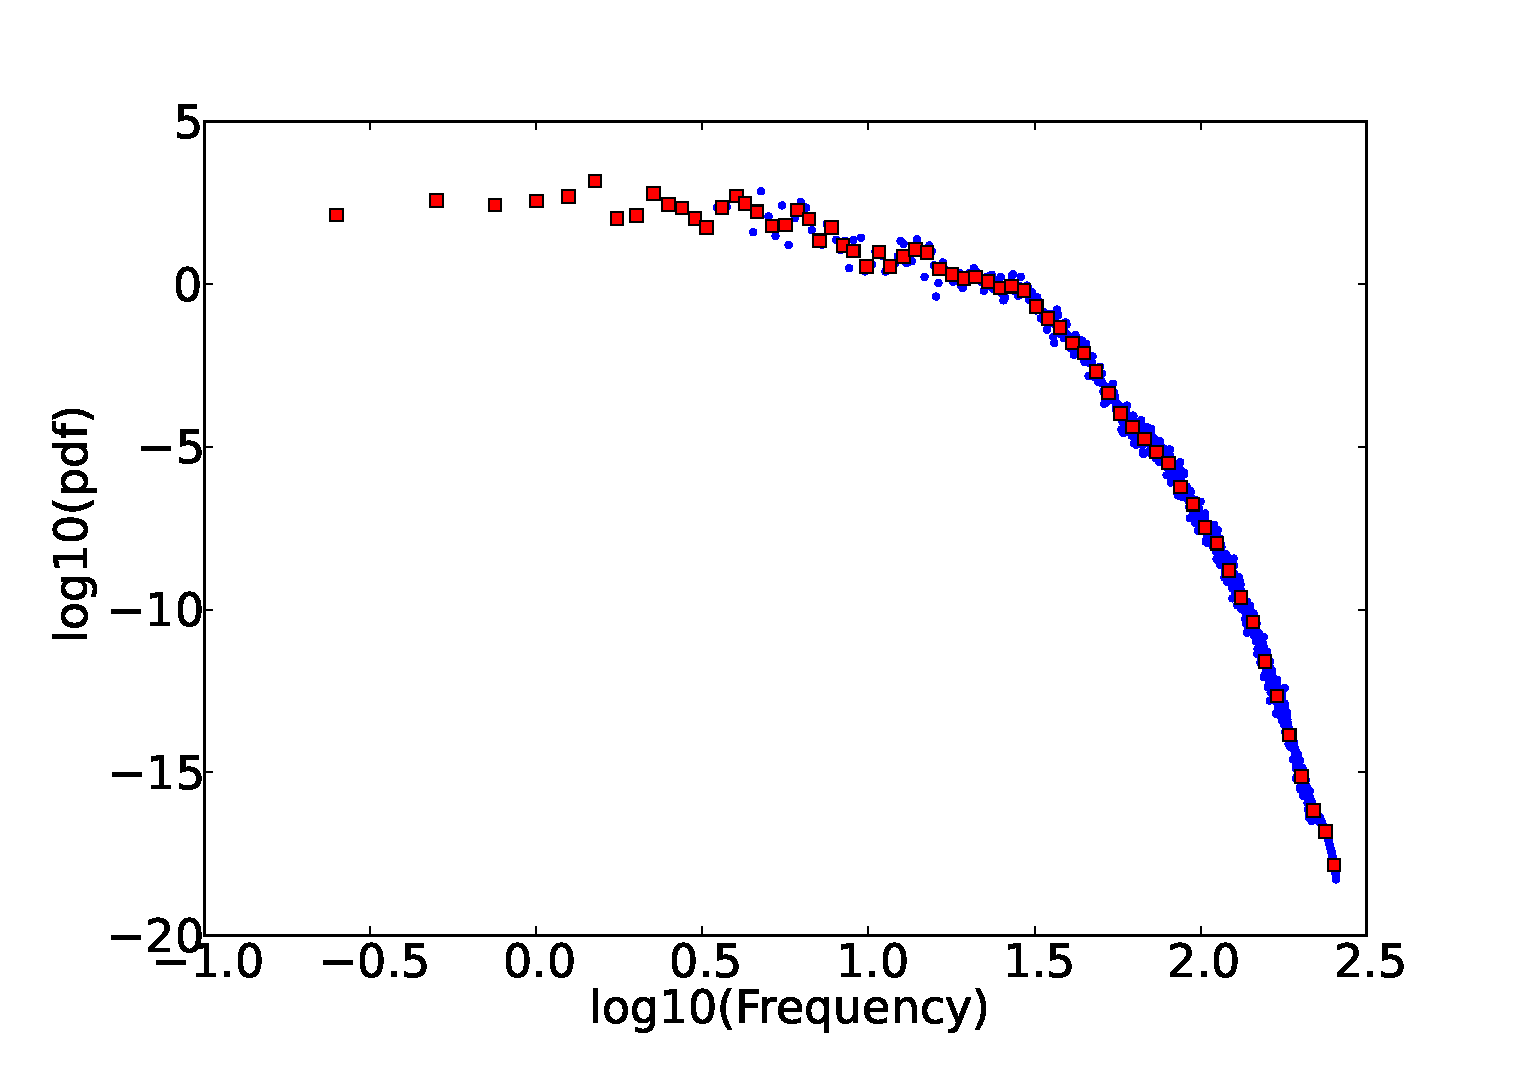
\epsfig{file = Figures/figure1.eps, width = 8cm}}
\caption{In double logarithmic scale, the original 1024 bins (blue dots) of the probability density function (pdf) obtained from averaging the \emph{n} power spectra of one recording, and the resulting quantized pdf with a resolution of 65 log-bins (red). The quantized pdf preserves very well the structure of the original, 1024-point pdf. }
\label{binnedEEGpowerspec}
\vspace{-0.1cm}
\end{figure}

%In summary, we build a probability density function of frequencies captured by the EEG scanning device from all the power spectra in a recording. We then use logarithmically-spaced bins to reduce the original 1024 frequency values to a smaller number of bins (e.g., 100 log-bins in \ref{binnedEEGpowerspec}). This method produces a statistical average of a time series, compressed into a single feature vector that it is easy to use in a classifier.


\subsection{Binary BCI Classifier}

To test the performance of the quantization method, we build a binary BCI using a support vector machine (SVM) classifier, which we train individually on each subject's recordings while varying the bin size. We use LinearSVC \cite{fan_liblinear:_2008}, a wrapper for LibLinear exposed in Python through the scikit-learn library \cite{pedregosa_scikit-learn:_2011}. We chose LinearSVC because BCI classification problems are generally presumed to be linear  \cite{garrett_comparison_2003,lotte_review_2007}, and because LibLinear's underlying C implementation boasts among the fastest train- and test-time performance among state-of-the-art solutions \cite{fan_liblinear:_2008}. We use a hyperparameter of 100, found through a grid-search of a randomly-selected sample of our dataset. We use scikit-learn's built-in cross-validation toolkit, which performs seven cross-validation steps utilizing different splits of data in each round.

Out of the seven mental gestures in the dataset, we want to identify and select, for each individual subject, the two gestures (or \textit{classes}) that we can most reliably differentiate from one another. This results in a personalized, binary classifier, where the SVM can discriminate between two mental gestures performed by the subject with the highest classification accuracy. The gesture pairs may vary from subject to subject. For example, one subject's best-case pair may be \textit{song} and \textit{sport} while another's may be \textit{color} and \textit{finger}. Subjects can then select one of two options by performing one of the mental gestures in their gesture pair.

\section{\uppercase{The effect of quantization technique on classifier speed and accuracy}}
\label{sec:quantization_eval}


Generally, we seek to maxmize our system's classification accuracy while minimizing its computational expense. One way to reduce the computational requirements of a SVM classifier is to reduce the size of the feature vectors on which it is trained and tested. Our signal quantization method allows us to directly adjust the size of feature vectors by changing the signal's resolution (see 3.1), though lowering the resolution of feature vectors could negatively effect the classifier's performance.

In this experiment, we examine the effect of resolution, operationalized by the number of bins used in the quantization step, on our BCI's performance, operationalized by the SVM's training time and by the SVM's estimated accuracy. 

H1: SVM accuracy will decrease with resolution.
H2: SVM training time will decrease with resolution.

\subsection{Protocol}

For each subject, we generate every pair of two tasks and cross-validate our SVM seven times on the recordings for this pair of tasks. We vary the resolution of the samples we feed to the SVM. For every task pair processed, we record mean classification accuracy across all rounds of cross-validation. For each subject, we record the best-performing taskpair, which corresponds to our estimation of optimal performance of the BCI for that subject.

As an additional performance audit, we measure the time needed to fit an SVM to the data for two randomly selected taskpairs across all subjects. We repeat this process ten thousand times at different resolutions, collecting the minimum time observed in each series of attempts.

\subsection{Results}

\begin{figure}

\begin{subfigure}%[!h]
  % \vspace{-0.2cm}
  % \centering
   {\epsfig{file = Figures/acc-bins.png, width = 8cm}}
  \caption{Mean best-case accuracy among all subjects compared to data resolution. At reoslutions of 100 points and greater, we find no evidence of an increase in classification accuracy. }
  \label{fig:fig1a}
  % \vspace{-0.1cm}
 \end{subfigure}

 \begin{subfigure}[b]%[!h]
  % \vspace{-0.2cm}
  % \centering
   {\epsfig{file = Figures/traintime-bins.png, width = 8cm}}
  \caption{Log of mean classifier training time compared to log of data resolution. The time needed to train the classifier increases logarithmically with resolution.}
  \label{fig:fig1b}
  % \vspace{-0.1cm}
 \end{subfigure}

 \begin{subfigure}%[!h]
  % \vspace{-0.2cm}
  % \centering
   {\epsfig{file = Figures/acc-traintime.png, width = 8cm}}
  \caption{ Best-case accuracy compared to the time needed to train the classifier. By decreasing the number of bins in the EEG data, we can decrease the time needed to train the support vector machine up to nine times without without significant detriment to classifier accuracy. }
  \label{fig:fig1c}
  % \vspace{-0.1cm}
 \end{subfigure}

 \end{figure}

We find support for H1. Although resolution was positively correlated with classifier accuracy (slope = .0013 R-squared = .773, p \textless .001), this effect appears only at resolutions lower than 100 points. We find no significant increase in SVM accuracy at resolutions over 100 bins. 

Resolution was also positively correlated with time to train classifier (slope = 0.5 R-squared = .947, p \textless .001). We compare accuracy and SVM training time directly in \ref{fig:fig1c}. Thus, we find support for H2.

Overall, we find that relatively small feature vectors produced with our method (100 values) yield classifiers as accurate as full-resolution samples (1024 values), and that reducing vector size in this way can dramatically increase the computational speed of training an SVM. 
\section{\uppercase{Opportunistic strategy for calibrating a binary BCI}}
\label{sec:calibration_eval}

In the previous experiment, we found that our compression technique can speed up an SVM classifier without significant detriment to BCI accuracy. However, for the technique to be useful in real-world applications, it must also allow users to quickly calibrate the system to their personal physiological signals.

In this experiment, we evaluate an opportunistic strategy for user calibration. Using a resolution of 100 points identified as optimal in the previous experiment, we measure user calibration time (the time it takes a user to achieve a threshold accuracy with the BCI) and the classification accuracy each user achieves after calibration. We hypothesize that this technique will allow for faster calibration than an exhaustive search (720 seconds) while maintaining sufficient system accuracy across users.

\subsection{Protocol}

As a baseline, we perform an exhaustive search of SVM accuracy on taskpairs identified each subject's best-performing taskpair. We recorded the frequency of each task's occurrence in a best-case taskpair \ref{table:name}. We used these data to inform the order in which our opportunistic calibration strategy would prompt the user to record tasks.

We begin with examples of the three tasks most commonly associated with best-case performance (base, pass, color) for an initial user calibration time of 120 seconds. We then perform a seven-fold cross-validation on every permutation of two of these tasks (base versus task, pass versus task, pass versus color, etc). The taskpair with the highest mean score across cross-validation rounds is selected for an additional testing session, in which the reamining 80 seconds of recordings for both tasks are used to generate an estimate of the classifier's accuracy on new EEG signals.

% this is where i put a table of tasks correlated with bestcase performance and a quick description, how we generated those data and what we need them for

\begin{table}[!h]
  \vspace{-0.2cm}
  \centering
  \begin{tabular}{ | l | l | l | p{5cm} |}
  \hline
  Task & Freq Bestcase \\ \hline
  Color & 10 \\ \hline
  Base & 5 \\ \hline
  Pass & 4 \\ \hline
  Sport & 3 \\ \hline
  Finger & 2 \\ \hline
  Song & 2 \\ \hline
  Eye & 2 \\ \hline
  \end{tabular}
  \caption{An exhaustive search of SVM accuracy on taskpairs identified each subject's best-performing taskpair. We recorded the frequency of each task's occurrence in a best-case taskpair, shown here. We used these data to inform the order in which our opportunistic calibration strategy would prompt the user to record tasks.}
  \label{table:name}
  \vspace{-0.1cm}
\end{table}

If the score on this additional testing round is below 75\% (a threshold for BCI literacy) \cite{vidaurre_towards_2010}, the user records sixty seconds of the taskpair next most correlated with bestcase accuracy across users. We repeat the above process on unexplored taskpairs repeated until a taskpair acheives over 75\% accuracy on post-calibration data, or until all taskpairs have been evaluated.

H1: We hypothesize that the opportunistic calibration strategy will reach threshold accuracy in less  time than will the exhaustive search.

H2: We hypothesize that the opportunistic strategy will acheive lower accuracy than will the exhaustive method, as it could find local optima.

\subsection{Results}

\begin{figure}[!h]
  \vspace{-0.2cm}
  \centering
   {\epsfig{file = Figures/3.png, width = 5.5cm}}
  \caption{Calibration time across subjects (top) and classifier accuracy (bottom). The vast majority of subjects acheive acceptable accuracy in under five minutes of training, and all subjects acheive BCI literacy in under 15 minutes. }
  \label{fig:fig2}
  \vspace{-0.1cm}
\end{figure}

A baseline exhaustive search required 2520 seconds of calibration time and produced an average accuracy of 92.5\% (\textit{$\sigma$} = .09) across subjects . Our opportunistic strategy took an average of 225.3 seconds of calibration time (\textit{$\sigma$} = 52.2) and produced an average accuracy of 88.3\% (\textit{$\sigma$} = .11).

We find that our strategy calibrates users to BCI control significantly more quickly than an exhaustive search (\textit{p} \textless .001 ). Thus, we find support for H1. Further, we do not a statistically significant difference in per-user accuracy between an opportunistic strategy and an exhaustive search (\textit{p} = .264). Thus, we find no support for H2.


\section{\uppercase{Discussion}}

\noindent We find that logarithmic binning dramatically decreases the computational expense of EEG-based calibration and classification without a significant detriment to accuracy. Further, we find that this technique is compatible with a training strategy capable of reaching acceptable classification rates with only a few minutes of training time. Since we used generallylow-cost, consumer hardware, our technique could make commercial BCI more feasible. 

The conclusions to be drawn from this study are limited in a few regards. First, calibration and classification were performed offline, so factors involving the user interface (such as feedback) are not taken into account. We cannot be sure, for instance, that our findings with short splices of ten-recordings data will persist when a system solicits recordings of only a second or under. Furthermore, a few of our tasks (e.g. the color task) relied on exogenous stimuli, which may be impractical in naturalistic settings for ergonomic reasons. Finally, we did not compare our findings to traditional signal processing methods in EEG.

Logarithmic binning could enable co-adaptive, online BCI with as few as one dry EEG sensor, making online calibration much more performant on mobile or embedded processors with limited computational resources. Alternatively, since logarithmic binning dramatically decreases the size of data fed to the classification algorithm, the technique could allow calibration to occur “in the cloud” - the BCI could pre-process the data on board, bin it, and ship this data to a more powerful server, which could process it online. By some combination of cloud-based and on-board processing, BCIs could gain from the accuracy of computationally expensive analytics without having to perform these computations on-board.

Future work could implement a system that calibrates a BCI online. Due to the small size of binned EEG signals, such a system could use a client/server architecture in which expensive processing (such as training multiple SVMs) is offloaded from the user’s system to a more powerful processor in teh cloud. This system could be used for the calibration of direct-control BCIs by attempting to find groups of tasks for which the classifier has high discriminatory power. A similar system could be used for long-term, affective recordings as well.

By collecting EEG data in the wild, we hope to discover more about how the mind behaves outside of laboratory environments. A particular interest is the non-stationary nature of neural recordings. By analyzing chronic EEG recordings at scale, we hope to make observations about how EEG signals change their expression over time, which could enable us to build more accurate BCIs that require less frequent re-calibration.

%\vfill
\bibliographystyle{apalike}
{\small
\bibliography{references}}

\vfill
\end{document}

